\documentclass[11pt]{article}


%%%%%%%%%%%%%%%%%%%%%%%%%%%%%%%%%%%%%%%%%%%%%%%%%%%%%%%%%%%%%%%%%%%%%%%%%%%%%%%%%%%%%%
%%%%%%%%%%%%%%%%%%% YOU PROBABLY DON"T NEED TO CHANGE ANYTHING HERE %%%%%%%%%%%%%%%%%%%
\usepackage[numbers,sort]{natbib}
\usepackage{amsfonts, amsmath}
\usepackage{graphicx}
\usepackage{libertine}
\usepackage{fullpage}
\usepackage{hyperref}
\hypersetup{
    colorlinks = true,
    linkcolor = blue,
    urlcolor  = blue,
    citecolor = blue,
    anchorcolor = blue}
\urlstyle{same}
%%%%%%%%%%%%%%%%%%%%%%%%%%%%%%%%%%%%%%%%%%%%%%%%%%%%%%%%%%%%%%%%%%%%%%%%%%%%%%%%%%%%%%
%%%%%%%%%%%%%%%%%%%%%%%%%%%%%%%%%%%%%%%%%%%%%%%%%%%%%%%%%%%%%%%%%%%%%%%%%%%%%%%%%%%%%%

% extra packages used by this report
\usepackage{amssymb}
\usepackage{booktabs}
\usepackage{float}

% no paragraph indentation; use a blank line between paragraphs instead
\setlength{\parindent}{0pt}
\setlength{\parskip}{0.4em}


%
% ===== DOCUMENT STARTS HERE =======
%
\begin{document}

\title{The Effects of Rotation \& Effective Dimension on Bayesian Optimisation \& CMA-ES Performance under a Fixed Evaluation Budget}
\date{\today}
\maketitle

{\bf Group Composition:}
\begin{enumerate}
\item Joanne Thomas, A0282542E, joanne.thomas@u.nus.edu
\item Shyann Loh, A0281432L, e1155560@u.nus.edu
\item Sruthi Babukumar, A0281495U, e1155623@u.nus.edu
\end{enumerate}

{\bf Github Repository:} \url{https://github.com/joanne-1234/dsa4212-assignment}

%
%
\section{Introduction}

Black-box optimisation finds good solutions when objective functions can be evaluated, but gradient information is often unavailable or impractical to obtain. When evaluations are expensive, an algorithm must use a limited evaluation budget effectively. Gaussian-process Bayesian optimisation (GP-BO) builds a probabilistic model from previous results to choose the next input. The Covariance Matrix Adaptation Evolution Strategy (CMA-ES) instead adjusts its search distribution based on groups of evaluated candidates (Frazier, 2018; Hansen, 2023).

The difficulty of black-box optimisation problems depends not only on the number of input variables but also on the structure of the objective function. A problem may have many input variables (a high ambient dimension) but a low effective dimension, meaning that the objective depends on only a small number of independent directions. These directions need not align with the original coordinate axes; rotation can change their orientation without changing the number of important directions. Previous research has studied and exploited such low-dimensional structure in BO, including important directions that do not align with individual coordinates (Wang et al., 2016; Li et al., 2016).

We aim to investigate how rotation affects the relative performance of GP-BO and CMA-ES across different effective dimensions under a fixed evaluation budget. Synthetic weighted-quadratic functions are constructed to isolate the effects of rotation and effective dimensionality on black-box optimisation performance while keeping the ambient dimension fixed. Established benchmarking practices, such as the COCO/BBOB suite, which investigates optimisation difficulties using separable and rotated functions (Hansen et al., 2009), motivate this design choice.

We evaluate both algorithms across multiple random rotations and independent runs, using random search as a baseline. Performance is assessed by the best objective value achieved within the evaluation budget. In summary, the study aims to characterise how algorithm performance varies across these controlled conditions, rather than to generalise beyond the functions and settings tested.

\section{Methods and Related Research}

\subsection{Gaussian-Process Bayesian Optimisation}

\subsubsection{Background: Gaussian-Process Bayesian Optimisation}

GP-BO uses a Gaussian process as a surrogate model to approximate an objective function based on previous evaluations providing predictive means and uncertainty estimates for unevaluated points (Frazier, 2018). 

The choice of covariance kernel influences how the GP models relationships between inputs. The study compares two RBF kernel variants: isotropic and Automatic Relevance Determination (ARD). The isotropic RBF kernel measures similarity based on Euclidean distance. Since Euclidean distances are preserved under rotation, the isotropic RBF kernel is rotation-invariant (Rasmussen \& Williams, 2006). However, this does not guarantee rotation invariance of the overall GP-BO algorithm due to factors such as search boundaries and acquisition optimisation. Alternatively, the Automatic Relevance Determination (ARD) kernel assigns a separate length scale to each coordinate. It is generally not rotation-invariant as rotation changes how variation is represented across coordinates. Comparison between the two kernels would provide further insight into how kernel parameterisation influences performance across axis-aligned and rotated objectives.

GP-BO uses an acquisition function to determine the next point to evaluate based on the GP’s predictions. We use Expected Improvement (EI), which scores each candidate by how much it is expected to improve on the best value observed so far (Frazier, 2018). The GP is updated after each evaluation until the evaluation budget is exhausted.

\subsubsection{Related Work: Low Effective Dimensionality}

Exploiting the low effective dimensionality of objective functions is an active area of research. Methods that actively learn a low-dimensional linear embedding alongside the objective function have been proposed (Garnett et al., 2013). These methods enable GP models to exploit important directions within a high-dimensional input space, even when these directions do not align with the original coordinate axes. Similarly, Moriconi et al.\ (2020) proposed learning a low-dimensional feature space jointly with the response surface and a reconstruction mapping, allowing BO to optimise within the lower-dimensional space.

\subsection{CMA-ES}

\subsubsection{Background: Covariance Matrix Adaptation Evolution Strategy}

CMA-ES searches by sampling a population of candidate inputs from a multivariate normal distribution. At generation $g$, candidates are sampled as
\begin{align}
\label{eq:cmaes}
x_k^{(g)} \sim \mathcal{N}\!\left(m^{(g)},(\sigma^{(g)})^2 C^{(g)}\right),\qquad k=1,\ldots,\lambda,
\end{align}
where $m$ is the search centre, $\sigma$ controls the overall spread, $C$ controls the shape and orientation, and $\lambda$ is the population size. After evaluating and ranking the candidates, CMA-ES moves the centre towards a weighted average of the better candidates. It updates the covariance matrix using current and past search steps, while adapting the step size to control the overall search scale (Hansen, 2023).

By adapting its full covariance, CMA-ES can stretch and rotate its search distribution along useful directions, including combinations of input coordinates (Hansen and Ostermeier, 2001; Hansen, 2023). Although CMA-ES is theoretically rotation-invariant under appropriate conditions (Hansen, 2023), the fixed axis-aligned bounds in our experiment may influence its observed rotation sensitivity.

\subsubsection{Related Work: Low Effective Dimensionality}

Rotation invariance does not guarantee that CMA-ES efficiently exploits low effective dimensionality. Uchida et al. (2024) identify inefficiencies arising from ambient-dimension-dependent parameters and step-size adaptation involving irrelevant directions. Their proposed CMA-ES-LED addresses these limitations and improves performance on the tested low-effective-dimensional problems.

Relative performance also depends on the evaluation budget. Loshchilov and Hutter (2016) highlight that BO methods often perform favourably under smaller budgets, whereas CMA-ES can benefit from larger budgets. Similarly, Santoni et al.\ (2024) benchmarked high-dimensional BO algorithms against standard BO, CMA-ES, and random search across the BBOB functions. Their findings showed that relative performance varied with evaluation budget, dimension and function landscape.

\subsection{Random Search as a Baseline}

Random search samples candidate solutions independently and uniformly from a predefined search domain. Unlike GP-BO and CMA-ES, it does not use previous evaluations to guide subsequent sampling. It provides a non-adaptive baseline for evaluating GP-BO and CMA-ES across effective dimensions and orientations (Bergstra \& Bengio, 2012).

\section{Experimental Design and Setup}

\subsection{Research Hypotheses}

We investigate how rotation affects the relative performance of GP-BO and CMA-ES, and whether this effect depends on effective dimension, under a budget of 400 objective evaluations per run. This motivates three hypotheses:
\begin{itemize}
\item \textbf{H1 (rotation):} ARD-BO will experience a larger rotation penalty than CMA-ES. ARD assigns a separate length scale to each input coordinate, whereas CMA-ES can adapt the orientation of its search distribution through a full covariance matrix, allowing it to model correlations between coordinates (Hansen, 2023).
\item \textbf{H2 (effective dimension):} ARD-BO's rotation penalty will be greater at smaller effective dimensions. In aligned settings, more coordinates are irrelevant, allowing ARD to down-weight them through larger length scales (Rasmussen \& Williams, 2006).
\item \textbf{H3 (kernel comparison):} ARD-BO will experience a larger rotation penalty than isotropic BO. Rotation is expected to reduce ARD's benefit from learning separate length scales for individual coordinates.
\end{itemize}

Random search provides a reference for orientation effects arising without adaptive search. All methods use the same bounded domain and evaluation budget. Because the search box remains fixed when the objective rotates, sampling geometry and boundary handling may also contribute to the observed effects.

\subsection{Objective Function}

All methods minimise weighted quadratics on $[-1,1]^D$, with ambient dimension $D=20$ and effective dimension $d\in\{2,5,10,15,20\}$:
\begin{align}
\label{eq:objective}
f(x)=\sum_{i=1}^{d}w_i(z_i-a_i)^2,\qquad z=x\ \text{(aligned)},\quad z=Q^\top x\ \text{(rotated)}.
\end{align}
Only the first $d$ coordinates of $z$ affect the objective. All methods search over the full 20-dimensional domain without using information about the active directions.

Weights are geometrically spaced from 1 to 100 and normalised to sum to one, introducing a 100-fold range in active-direction curvature. The shift $a \in \mathbb{R}^d$ is drawn from a standard normal distribution and rescaled to have Euclidean norm 0.5. This places a minimiser inside the box, at distance 0.5 from the origin, in either orientation, while keeping the box centre non-optimal. The minimum value is zero, with infinitely many minimisers when $d < 20$ and a unique minimiser when $d = 20$.

The orthogonal matrix $Q$ is generated by QR decomposition of a Gaussian random matrix, with Mezzadri's (2007) diagonal-sign correction and an additional correction to ensure its determinant is $+1$, giving a proper rotation rather than a reflection. Each matched pair of aligned and rotated objectives uses the same problem seed, weights and shift, while the search box remains fixed.

\subsection{Algorithm Configurations}

\textbf{Gaussian-process Bayesian optimisation.} The two GP-BO variants share the same optimisation procedure and differ only in their covariance kernel. Both use an RBF kernel multiplied by a constant kernel, allowing the signal variance to be learned. Isotropic BO uses a single shared length scale across all 20 input coordinates, whereas ARD-BO fits 20 separate length scales, one for each coordinate. The GP hyperparameters are optimised during fitting, with one optimiser restart. The fitted kernel parameters initialise the subsequent fit.

Both variants use EI as the acquisition function for minimisation, with an exploration parameter of $\xi = 0.01$. The first 40 evaluations are obtained from a uniform random initial design over the search domain. For each subsequent evaluation, the objective values are standardised, and the GP is then fitted to the observations. EI is then evaluated over a newly generated set of 2,048 uniformly sampled candidates, and the candidate with the highest EI is selected. A numerical jitter of $10^{-8}$ is used in GP fitting.

\textbf{CMA-ES.} We use CMA-ES with a population size of 12 and an initial step size of $\sigma_0 = 0.3$. The initial search distribution is centred at the origin with an initially spherical covariance structure. Full covariance adaptation and active covariance updates are enabled from the start. Finally, box constraints are handled by pycma's \texttt{BoundTransform} boundary handler.

\textbf{Random search.} At each evaluation, candidates are sampled independently and uniformly from the full domain $[-1, 1]^{20}$.

\subsection{Evaluation Protocol}

For each of the five effective dimensions, we use five problem seeds (0--4), two orientations (aligned and rotated) and two method seeds (100 and 101), giving 100 runs per method. Problem seeds determine the objective's shift and rotation, while method seeds control the algorithm's randomness. Each run has a budget of 400 objective evaluations, including any initial evaluations, giving 160,000 evaluations across the four methods.

The same objective instances are used across all methods, with aligned and rotated runs matched by problem and method seed. For each method seed, the two BO variants share identical initial designs and candidate pools. These sampling streams and the random-search samples depend only on the method seed and therefore repeat across problem instances.

A supplementary experiment examines the role of coordinate-wise curvature in the relative performance of ARD and isotropic BO. It uses equal weights and a Hadamard-based rotation, giving equal curvature along all input coordinates in the rotated objectives. The effective dimensions, seeds, evaluation budget and BO settings remain unchanged, giving 100 additional runs per BO variant.

\subsection{Performance Measures}

We evaluate optimisation performance using the final best-so-far objective value, defined as the lowest value observed within 400 evaluations. For each effective dimension and orientation, performance is summarised by the median across 10 runs.

To quantify the effect of rotation, we calculate a rotation penalty using matched aligned and rotated runs. For each effective dimension, problem seed and method seed, the log-ratio between the final best values is defined as
\begin{align}
\label{eq:logratio}
r=\log\!\left(\frac{f_{\mathrm{rotated}}^{\mathrm{best}}}{f_{\mathrm{aligned}}^{\mathrm{best}}}\right).
\end{align}
A positive value indicates worse performance after rotation, while a negative value indicates improved performance. A value of zero indicates no difference. To avoid taking the logarithm of zero, a numerical floor of $10^{-12}$ is applied to the final best values.

The two method-seed log-ratios in Equation \eqref{eq:logratio} are averaged within each problem seed, then averaged across the five problems. The geometric-mean rotation penalty is defined as $P = \exp(\bar r)$, where $\bar r$ is the overall mean log-ratio. A penalty greater than one indicates worse performance after rotation, while a value below one indicates improvement. The rotation-penalty figure displays $\log_{10}P$, where zero indicates no overall difference between aligned and rotated performance.

\section{Results and Discussion}

\subsection{Performance across Effective Dimensions}

Under the tested conditions, ARD-BO achieves the lowest median best-so-far objective values at $d = 2$ in both orientations and at $d = 5$ when aligned. However, CMA-ES performs best at rotated $d = 5$ and at higher effective dimensions ($d \geq 10$) in both orientations. Although its final objective values increase with effective dimension, they increase less sharply than those of the GP-BO variants. At $d = 20$, CMA-ES achieves nearly an order of magnitude lower final values ($\sim 4 \times 10^{-3}$ versus $\sim 3$--$4 \times 10^{-2}$), as shown in Figure \ref{fig:performance}.

%
% === PERFORMANCE FIGURE ===
%
\begin{figure}[H]
\centering
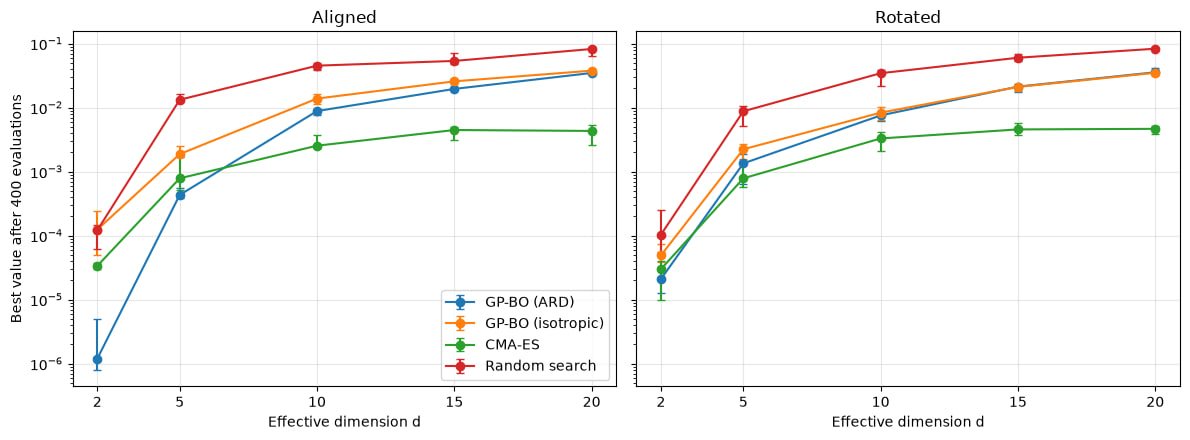
\includegraphics[width=0.85\textwidth]{figures/img-000.jpg}
\caption{Median final best value after 400 evaluations against effective dimension.}
\label{fig:performance}
\end{figure}

Median runtimes were compared across algorithms and effective dimensions, pooling aligned and rotated runs (Table \ref{tab:runtime}).

\begin{table}[H]
\centering
\caption{Median runtime per run (seconds).}
\label{tab:runtime}
\begin{tabular}{lrrrrr}
\toprule
Method & $d=2$ & $d=5$ & $d=10$ & $d=15$ & $d=20$ \\
\midrule
GP-BO (ARD)       & 338.81 & 315.48 & 347.90 & 327.98 & 383.46 \\
CMA-ES            & 0.03   & 0.03   & 0.03   & 0.03   & 0.03   \\
GP-BO (isotropic) & 25.26  & 25.30  & 32.16  & 27.08  & 26.64  \\
Random search     & 0.01   & 0.01   & 0.01   & 0.01   & 0.01   \\
\bottomrule
\end{tabular}
\end{table}

GP-BO incurs additional computational overhead from Gaussian Process Regression (GPR). This overhead arises from hyperparameter optimisation and acquisition function maximisation (Frazier, 2018). ARD-BO takes approximately 13 times longer than isotropic BO, likely because it optimises 20 coordinate-specific length scales rather than one shared length scale (Tang et al., 2026). In contrast, CMA-ES has relatively low internal computational costs (Loshchilov \& Hutter, 2016), while random search requires no surrogate-model fitting.

Therein lies the trade-off between optimisation performance and computational cost:
\begin{itemize}
\item ARD-BO achieves lower final objective values than isotropic BO at low effective dimensions, but its advantage diminishes at higher dimensions and comes with greater computational cost.
\item CMA-ES is significantly faster than both BO methods and achieves the lowest final objective values at higher effective dimensions ($d = 10, 15, 20$).
\item Random search is the fastest method but generally produces the worst optimisation results under our experimental conditions.
\end{itemize}

While these runtimes and final objective values are specific to our implementation and computational environment, and should therefore be interpreted as an empirical comparison rather than an inherent performance guarantee for each algorithm, they highlight an important consideration when evaluating optimisation methods: the algorithm achieving the lowest final objective value may not necessarily be the most computationally efficient, particularly under a fixed evaluation budget.

\subsection{Effect of Rotation: H1--H3}

The results partially support H1. At low effective dimensions ($d = 2, 5$), ARD-BO has larger geometric-mean rotation penalties than CMA-ES: at $d = 2$, $\log_{10}P \approx 0.90$ for ARD-BO (roughly $8\times$ worse after rotation) compared with $-0.22$ for CMA-ES.

%
% === ROTATION FIGURE ===
%
\begin{figure}[H]
\centering
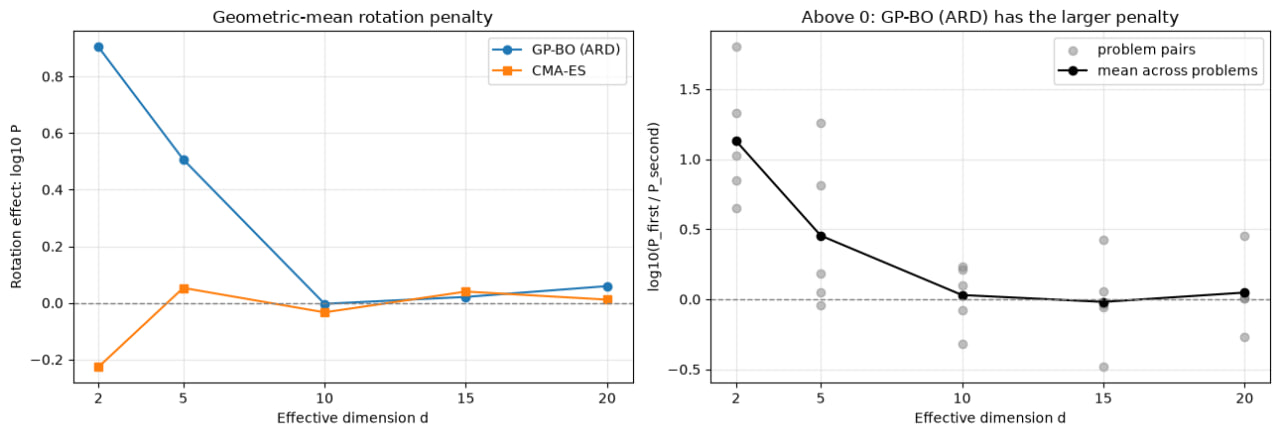
\includegraphics[width=0.85\textwidth]{figures/img-002.jpg}
\caption{Geometric-mean rotation effect for ARD-BO and CMA-ES, and per-problem penalty comparison.}
\label{fig:rotation}
\end{figure}

At $d = 5$, the penalties are approximately 0.50 ($3\times$ worse) and 0.05, respectively. The per-problem log-ratio, $\log_{10}(P_{\text{ARD-BO}}/P_{\text{CMA-ES}})$, tells the same story, with a mean of $\approx 1.1$ at $d = 2$ and $\approx 0.45$ at $d = 5$ (Figure \ref{fig:rotation}). This is consistent with the theoretical rotation invariance of CMA-ES, which adapts the full covariance matrix of its search distribution, allowing it to capture correlations between input dimensions and adjust to different orientations of the objective function (Hansen \& Ostermeier, 1996). However, the difference in rotation penalties becomes substantially smaller at higher effective dimensions ($d = 10, 15, 20$), and CMA-ES does not consistently exhibit a lower penalty across all dimensions. This suggests that its theoretical rotation invariance does not necessarily translate into identical empirical performance under the finite evaluation budgets and stochastic conditions of our experiments.

H2 is supported by the results as well. ARD-BO exhibits substantially greater rotation penalties at lower effective dimensions ($d = 2, 5$), while the $\log_{10}$ penalty falls close to 0 at higher dimensions. This may be explained by disruption of coordinate-wise sparsity following rotation. In aligned settings, fewer original coordinates influence the objective at lower effective dimensions, allowing ARD-BO to potentially exploit this structure through coordinate-specific length scales. Rotation distributes these influential directions across the original coordinates, making it more difficult for ARD-BO to determine which coordinates are relevant. At higher effective dimensions, more original coordinates are already influential, making the loss of coordinate-wise sparsity less pronounced.

H3 is supported at low effective dimensions. Using the median $\log_{10}$ rotation penalty across the 10 matched runs, ARD-BO records 1.25 at $d = 2$ (approximately $18\times$ worse after rotation) compared with $-0.49$ for isotropic BO, which improves after rotation. ARD-BO has a larger rotation penalty in all 10 matched runs at $d = 2$, and in 9 out of 10 runs at both $d = 5$ and $d = 10$. However, at $d = 15$ and $d = 20$, the median paired differences decrease to 0.07 and 0.01, respectively, indicating a much smaller difference between the methods. This pattern can be explained by the coordinate-specific length scales of ARD kernels. A large length scale means that the GP treats the objective as changing slowly along that coordinate, reducing the coordinate's influence on the model (Rasmussen \& Williams, 2006). Rotation spreads important directions across multiple coordinates, reducing this advantage. In contrast, isotropic BO uses a single shared length scale, and its covariance kernel is rotation-invariant because Euclidean distances are preserved (Rasmussen \& Williams, 2006). This makes its surrogate model less dependent on coordinate alignment, although the overall BO procedure may still be affected by rotation.

\subsection{Understanding ARD's Advantage}

Although ARD-BO exhibited larger rotation penalties than isotropic BO at lower effective dimensions, it still achieved a better final objective value on rotated problems. We investigated whether ARD's coordinate-specific length scales allowed it to retain an advantage after rotation by capturing differences in curvature across input coordinates. In the main experiment, unequal weights combined with random rotation produced uneven curvature across coordinates. To examine whether the unequal weights influenced the observed result, we repeated the experiment on an equal-curvature objective: the active directions were given equal weights and the rotation was built from a Hadamard matrix, so that every input has the same curvature after rotation.

The results suggest that ARD-BO's advantage in the main weighted experiment may partly depend on the objective's curvature structure. Its coordinate-specific length scales may help capture differences in curvature across directions, contributing to its lower final objective values than isotropic BO. At $d = 2$, ARD-BO achieves a lower median final objective value in the rotated weighted setting ($2.10 \times 10^{-5}$ versus $4.92 \times 10^{-5}$). However, under equal curvature, this advantage disappears, with isotropic BO outperforming ARD-BO ($2.07 \times 10^{-5}$ versus $2.91 \times 10^{-5}$). A similar pattern occurs at $d = 5$, where the two methods achieve approximately equal final objective values under equal curvature (Table \ref{tab:curvature}).

\begin{table}[H]
\centering
\caption{Median final best values for ARD-BO and isotropic BO on weighted and equal-curvature objectives.}
\label{tab:curvature}
\resizebox{\textwidth}{!}{%
\begin{tabular}{clrrrr}
\toprule
$d$ & Objective & Aligned: ARD & Aligned: isotropic & Rotated: ARD & Rotated: isotropic \\
\midrule
2 & Weighted        & 1.20e-06 & 1.24e-04 & 2.10e-05 & 4.92e-05 \\
2 & Equal curvature & 7.48e-06 & 1.08e-04 & 2.91e-05 & 2.07e-05 \\
5 & Weighted        & 4.33e-04 & 1.88e-03 & 1.34e-03 & 2.23e-03 \\
5 & Equal curvature & 1.23e-03 & 2.57e-03 & 2.08e-03 & 2.09e-03 \\
\bottomrule
\end{tabular}}
\end{table}

These findings support curvature as a possible contributor to ARD's advantage, although the supplementary experiment also changes the rotation construction.

\section{Limitations}

First, the experiments use weighted quadratic objectives, which do not represent more complex optimisation landscapes with multiple local minima. Rotating the objective within a fixed axis-aligned box also changes its interaction with the boundaries. Random search showed differences under rotation despite having no orientation-dependent model, suggesting possible boundary effects. Using a rotation-invariant domain, such as a ball, could help isolate these effects. Additionally, the supplementary experiment changes both weights and rotation, so curvature cannot be identified as the sole cause of ARD's advantage under rotation.

Second, only five problem instances were tested per effective dimension, with two runs per method on each instance. With such a limited sample, the results may be influenced by the particular shifts and rotations sampled rather than reflecting a general pattern. Rotation penalties close to one should therefore be interpreted cautiously, as they may reflect variation across instances rather than a consistent rotation effect.

Third, CMA-ES starts at the centre of the search box, while GP-BO uses 40 uniformly sampled initial points. Since the nearest minimiser of each problem lies 0.5 units from the centre, CMA-ES may benefit from starting relatively close to an optimum. This initialisation difference may therefore influence their relative performance, rather than the results reflecting only differences in their optimisation methods.

Finally, the results depend on the chosen hyperparameters and budget of 400 evaluations. GP-BO optimises expected improvement over 2,048 random candidates without local refinement, potentially missing promising points. Therefore, different budgets or settings could change the relative performance.

\section{Conclusion}

This study examined how rotation affects the performance of GP-BO and CMA-ES across effective dimensions under a fixed evaluation budget. ARD-BO achieved the best results at low effective dimensions, particularly for aligned objectives, while CMA-ES generally performed better at higher effective dimensions. H1 was partially supported, as ARD-BO showed greater rotation sensitivity than CMA-ES mainly at low effective dimensions. H2 was supported, with ARD-BO's rotation penalty decreasing as effective dimension increased. H3 was most strongly supported at low effective dimensions, where ARD-BO experienced larger rotation penalties than isotropic BO. The supplementary experiment further suggested that coordinate-wise curvature may contribute to ARD-BO's advantage on rotated objectives. Overall, the results highlight the importance of effective dimension, coordinate alignment and objective structure when comparing optimisation methods under a limited evaluation budget.

%
% === BIBLIOGRAPHY =====
%
\section*{References}
\begin{small}
\setlength{\parskip}{0.3em}

Bergstra, J., \& Bengio, Y. (2012). Random search for hyper-parameter optimization. \emph{Journal of Machine Learning Research}, 13, 281--305. \url{https://www.jmlr.org/papers/volume13/bergstra12a/bergstra12a.pdf}

Frazier, P. I. (2018). A tutorial on Bayesian optimisation (arXiv:1807.02811). arXiv. \url{https://doi.org/10.48550/arXiv.1807.02811}

Garnett, R., Osborne, M. A., \& Hennig, P. (2013). Active learning of linear embeddings for Gaussian processes (arXiv:1310.6740). arXiv. \url{https://doi.org/10.48550/arXiv.1310.6740}

Hansen, N. (2023). The CMA evolution strategy: A tutorial (arXiv:1604.00772). arXiv. \url{https://doi.org/10.48550/arXiv.1604.00772}

Hansen, N., Finck, S., Ros, R., \& Auger, A. (2009). Real-parameter black-box optimization benchmarking 2009: Noiseless functions definitions (INRIA Research Report No. RR-6829). INRIA. \url{https://inria.hal.science/inria-00362633}

Hansen, N., \& Ostermeier, A. (1996). Adapting arbitrary normal mutation distributions in evolution strategies: The covariance matrix adaptation. \emph{Proceedings of the 1996 IEEE International Conference on Evolutionary Computation (ICEC'96)}, 312--317.

Hansen, N., \& Ostermeier, A. (2001). Completely derandomized self-adaptation in evolution strategies. \emph{Evolutionary Computation}, 9(2), 159--195. \url{https://doi.org/10.1162/106365601750190398}

Li, C.-L., Kandasamy, K., P\'oczos, B., \& Schneider, J. (2016). High dimensional Bayesian optimisation via restricted projection pursuit models. \emph{Proceedings of the 19th International Conference on Artificial Intelligence and Statistics}, 884--892. \url{https://proceedings.mlr.press/v51/li16e.html}

Loshchilov, I., \& Hutter, F. (2016). CMA-ES for hyperparameter optimization of deep neural networks (arXiv:1604.07269). arXiv. \url{https://doi.org/10.48550/arXiv.1604.07269}

Mezzadri, F. (2007). How to generate random matrices from the classical compact groups. \emph{Notices of the American Mathematical Society}, 54(5), 592--604. \url{https://doi.org/10.48550/arXiv.math-ph/0609050}

Moriconi, R., Deisenroth, M. P., \& Kumar, K. S. S. (2020). High-dimensional Bayesian optimization using low-dimensional feature spaces (arXiv:1902.10675). arXiv. \url{https://doi.org/10.48550/arXiv.1902.10675}

Rasmussen, C. E., \& Williams, C. K. I. (2006). \emph{Gaussian processes for machine learning}. The MIT Press. \url{https://gaussianprocess.org/gpml/chapters/RW.pdf}

Santoni, M. L., Raponi, E., Leone, R. D., \& Doerr, C. (2024). Comparison of high-dimensional Bayesian optimization algorithms on BBOB (arXiv:2303.00890). arXiv. \url{https://doi.org/10.48550/arXiv.2303.00890}

Tang, W.-T., Muthyala, M., \& Paulson, J. A. (2026). Isotropic Gaussian processes improve vanilla Bayesian optimization in high dimensions (arXiv:2610.05780). arXiv. \url{https://doi.org/10.48550/arXiv.2610.05780}

Uchida, K., Yamaguchi, T., \& Shirakawa, S. (2024). Covariance matrix adaptation evolution strategy for low effective dimensionality (arXiv:2412.01156). arXiv. \url{https://doi.org/10.48550/arXiv.2412.01156}

Wang, Z., Hutter, F., Zoghi, M., Matheson, D., \& De Freitas, N. (2016). Bayesian optimization in a billion dimensions via random embeddings. \emph{Journal of Artificial Intelligence Research}, 55, 361--387. \url{https://doi.org/10.1613/jair.4806}

\end{small}

\end{document}
